\begin{table}
	\tbl{Locations where sensors were installed}
	{\begin{tabular}{clll} 
		\toprule
		 ID & Location & Type & Installation notes\\
		 \midrule
		 1 & Camden High Street & Phone Shop & Bus stop in front\\
		 2 & Central St.Giles Piazza & Restaurant & Seating area on both sides\\
		 3 & Holborn Underground Station & Information Kiosk & Overlooks station entrance\\
		 4 & Brunswick Center & Fast Food Restaurant & Has seating area on one side\\
		 5 & The Strand & Tea Shop & Has phone shop next door \\
		 \bottomrule
	\end{tabular}}
	\label{locations-table}
\end{table}

\begin{figure}
	\begin{center}
		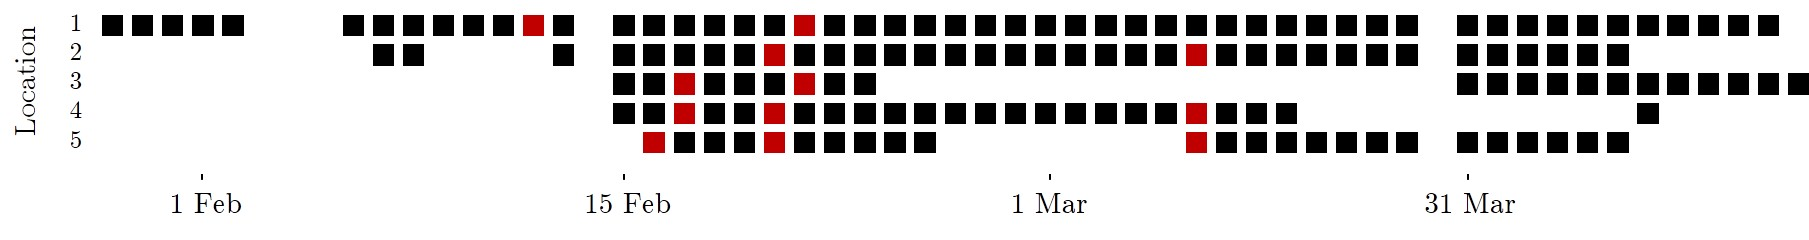
\includegraphics [width=0.90\linewidth] {images/main_schedule.jpeg}
		\caption{Days when the sensors were active at the corresponding location. The red square shows that manual data collection was also done.}
		\label{pilot_clustering}
	\end{center}
\end{figure}

The main study was designed to validate the results of the pilot study over different locations at different times. 
We choose five different locations across central London, to install the sensors and collect data for a long period of time. 
We also carry out manual counting on these locations along with this across different time of the day. 
We then apply the filtering based on signal strength and sequence numbers and compare with manual counts and evaluate the effectiveness of the process with the mean error per minute on these locations. 
Finally we calculate the ajustment factor for the first interval of manual counts and check if that works on the consecutive intervals. 

The locations where the data were collected are shown in the table. The location are chosen for their variety of configuration and sources of noise. Location 1 is the `cleanest' of while location 2 is the one with the most complexity. The configuration, installation and data collection schedule is shown in the figure. 

Though data was collected for many continous days, for the purposes of comparing with ground truth we just consider the only the data from sensors corresponding to those sessions. We have 12 sets of data over 6 different days. We have atleast two set manual counts for each location for verification of calibration.

\begin{figure}
	\centering
	\subfigure[Installation configuration of sensors at various locations]{
		\resizebox*{0.46\linewidth}{!}{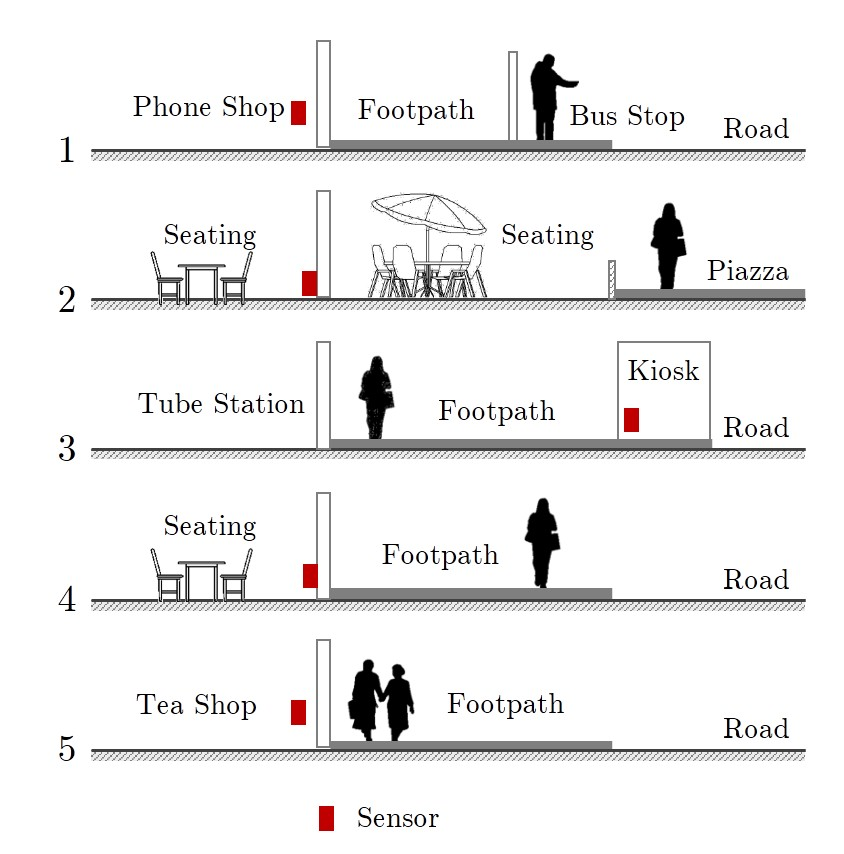
\includegraphics[trim=20 6 20 6,clip]{images/main_configs.jpeg}}}\hspace{20pt}
	\subfigure[Density distribution of signal strength (lower values show higher signal strength)]{
		\resizebox*{0.46\linewidth}{!}{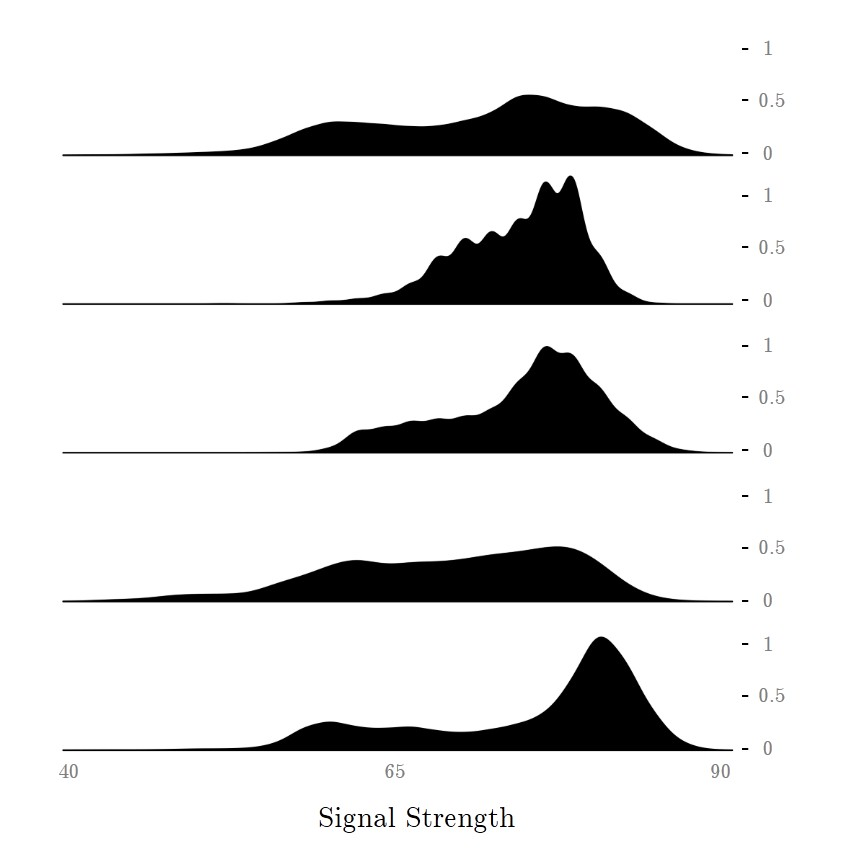
\includegraphics[trim=20 4 25 6,clip]{images/main_signals.jpeg}}}
	\caption{Distribution of signal strengths across locations} \label{methodology_schematic}
\end{figure}

First we see how the distribution of the signal strength varies with location and configuration. 
The density plot for signal strength is shown alogn with configuration in figure.
We can see that the signal strength distribution shows distinct patterns of high and low when the installation is that there is a clear distant source of noise but this distinction get more and more obscure as we move towards difficult installations. 
For example, location 2 is almost a normally distributed noise as it is too far to pick up any pedestrians but location 5 with a clear view of footpath and a phone shop next door shows clear distinction between the two. 
Intuitively the classfication algorithm should give us better results in the latter. 
It is important to note that we are dealing with relative singal strengths, this can vary with location and time of the analysis but we should be still be able to differentiate signal from noise. 
We run the kmeans classification algorithm and filter out the probe requests which are randomised and have signal strengths less than the second break (or the threshold). 
We then count the number of Unique MAC addresses present in every minute and remove MAC addreses which reappear within 30 minutes of previous appearance. 
We then compare this with the minute by minute aggreagation for the manual counts and find the average error per minute for the sensor count. 
The results are shown in the table.We see that the location 2 has the most error 400\% confirming our intuition while surprisingly location 3 has the least error -3\%. 
We also see that the error follows the complexity of the installation. 
It is also very promising that this method alone reduces our margin of error by a 50 - 100\%
For some practical purposes which do not require absolute numbers, this should be sufficient. 
e.g. Indexes of activity and change dashboards and short term trends identification.

We see that the success of the signal strength filtering depends on the how we tackle the problems in the installing the devices.
The more the device in installed in a way that the field of measurement is distinct from its surroundings (however noisy they might be) the more successful this process is.
Closer sources error causes overcounting as we see in 2, 4 but at the same time highly close field of measurement with no big source of error can cause undercounting such as in 3. The complexity of the installation and uniformity of surroundings near the sensors directly coorrelate to the MAPE.
The most effective way of measuring pedestrian is to have the sensor next to have the sensor next to clear area of pedestrian activity and in case of absence of any major source of noise, we should not do the signal strength filtering at all. We can even note the major possible sources of noise around the device and use it to fiugre out the right way of partitioning the data e.g. location 2 and 3 should have different pattern of signal strength filtering depending on their configuration.

In terms of filtering by sequence numbers we see that the the filtering works in all the locations. It has the similar effect as the signal strength and brings us furthe closer to the manual count. Finally we calculate the adjustment factor from the first 15 minutes and apply that for the rest of the interval. We get the counts down to almost 10\% on good locations. The locations which still over count are the ones with seating next to them (2 and 4). We also see that the trends are preserved with the filtering process.

\begin{table}
	\tbl{Data collected at different locations and the correspondin mean absolute percentage error after each filtering process}
	{\begin{tabular}{ccccccc} 
		\toprule
			Sensor & Signal strength & Adjustment & MAPE & MAPE after & MAPE after & MAPE of\\
			& threshold & factor & without any & filtering signal & filtering sequence & final adjusted\\
			& (-dBm) & &  cleaning (\%) & strength (\%) & numbers (\%) & counts (\%)\\
		 \midrule
			1 & -70 & 1.25 & 259 &  22 & -13 &  9 \\
			2 & -74 & 0.51 & 928 & 396 & 206 & 55 \\
			3 & -72 & 1.60 &  87 & -19 & -31 & 10 \\
			4 & -70 & 0.88 & 498 & 142 &  52 & 33 \\
			5 & -72 & 0.80 & 473 &  84 &  38 & 11 \\
		 \bottomrule
	\end{tabular}}
	\label{errors-table}
\end{table}

\begin{figure}
	\begin{center}
		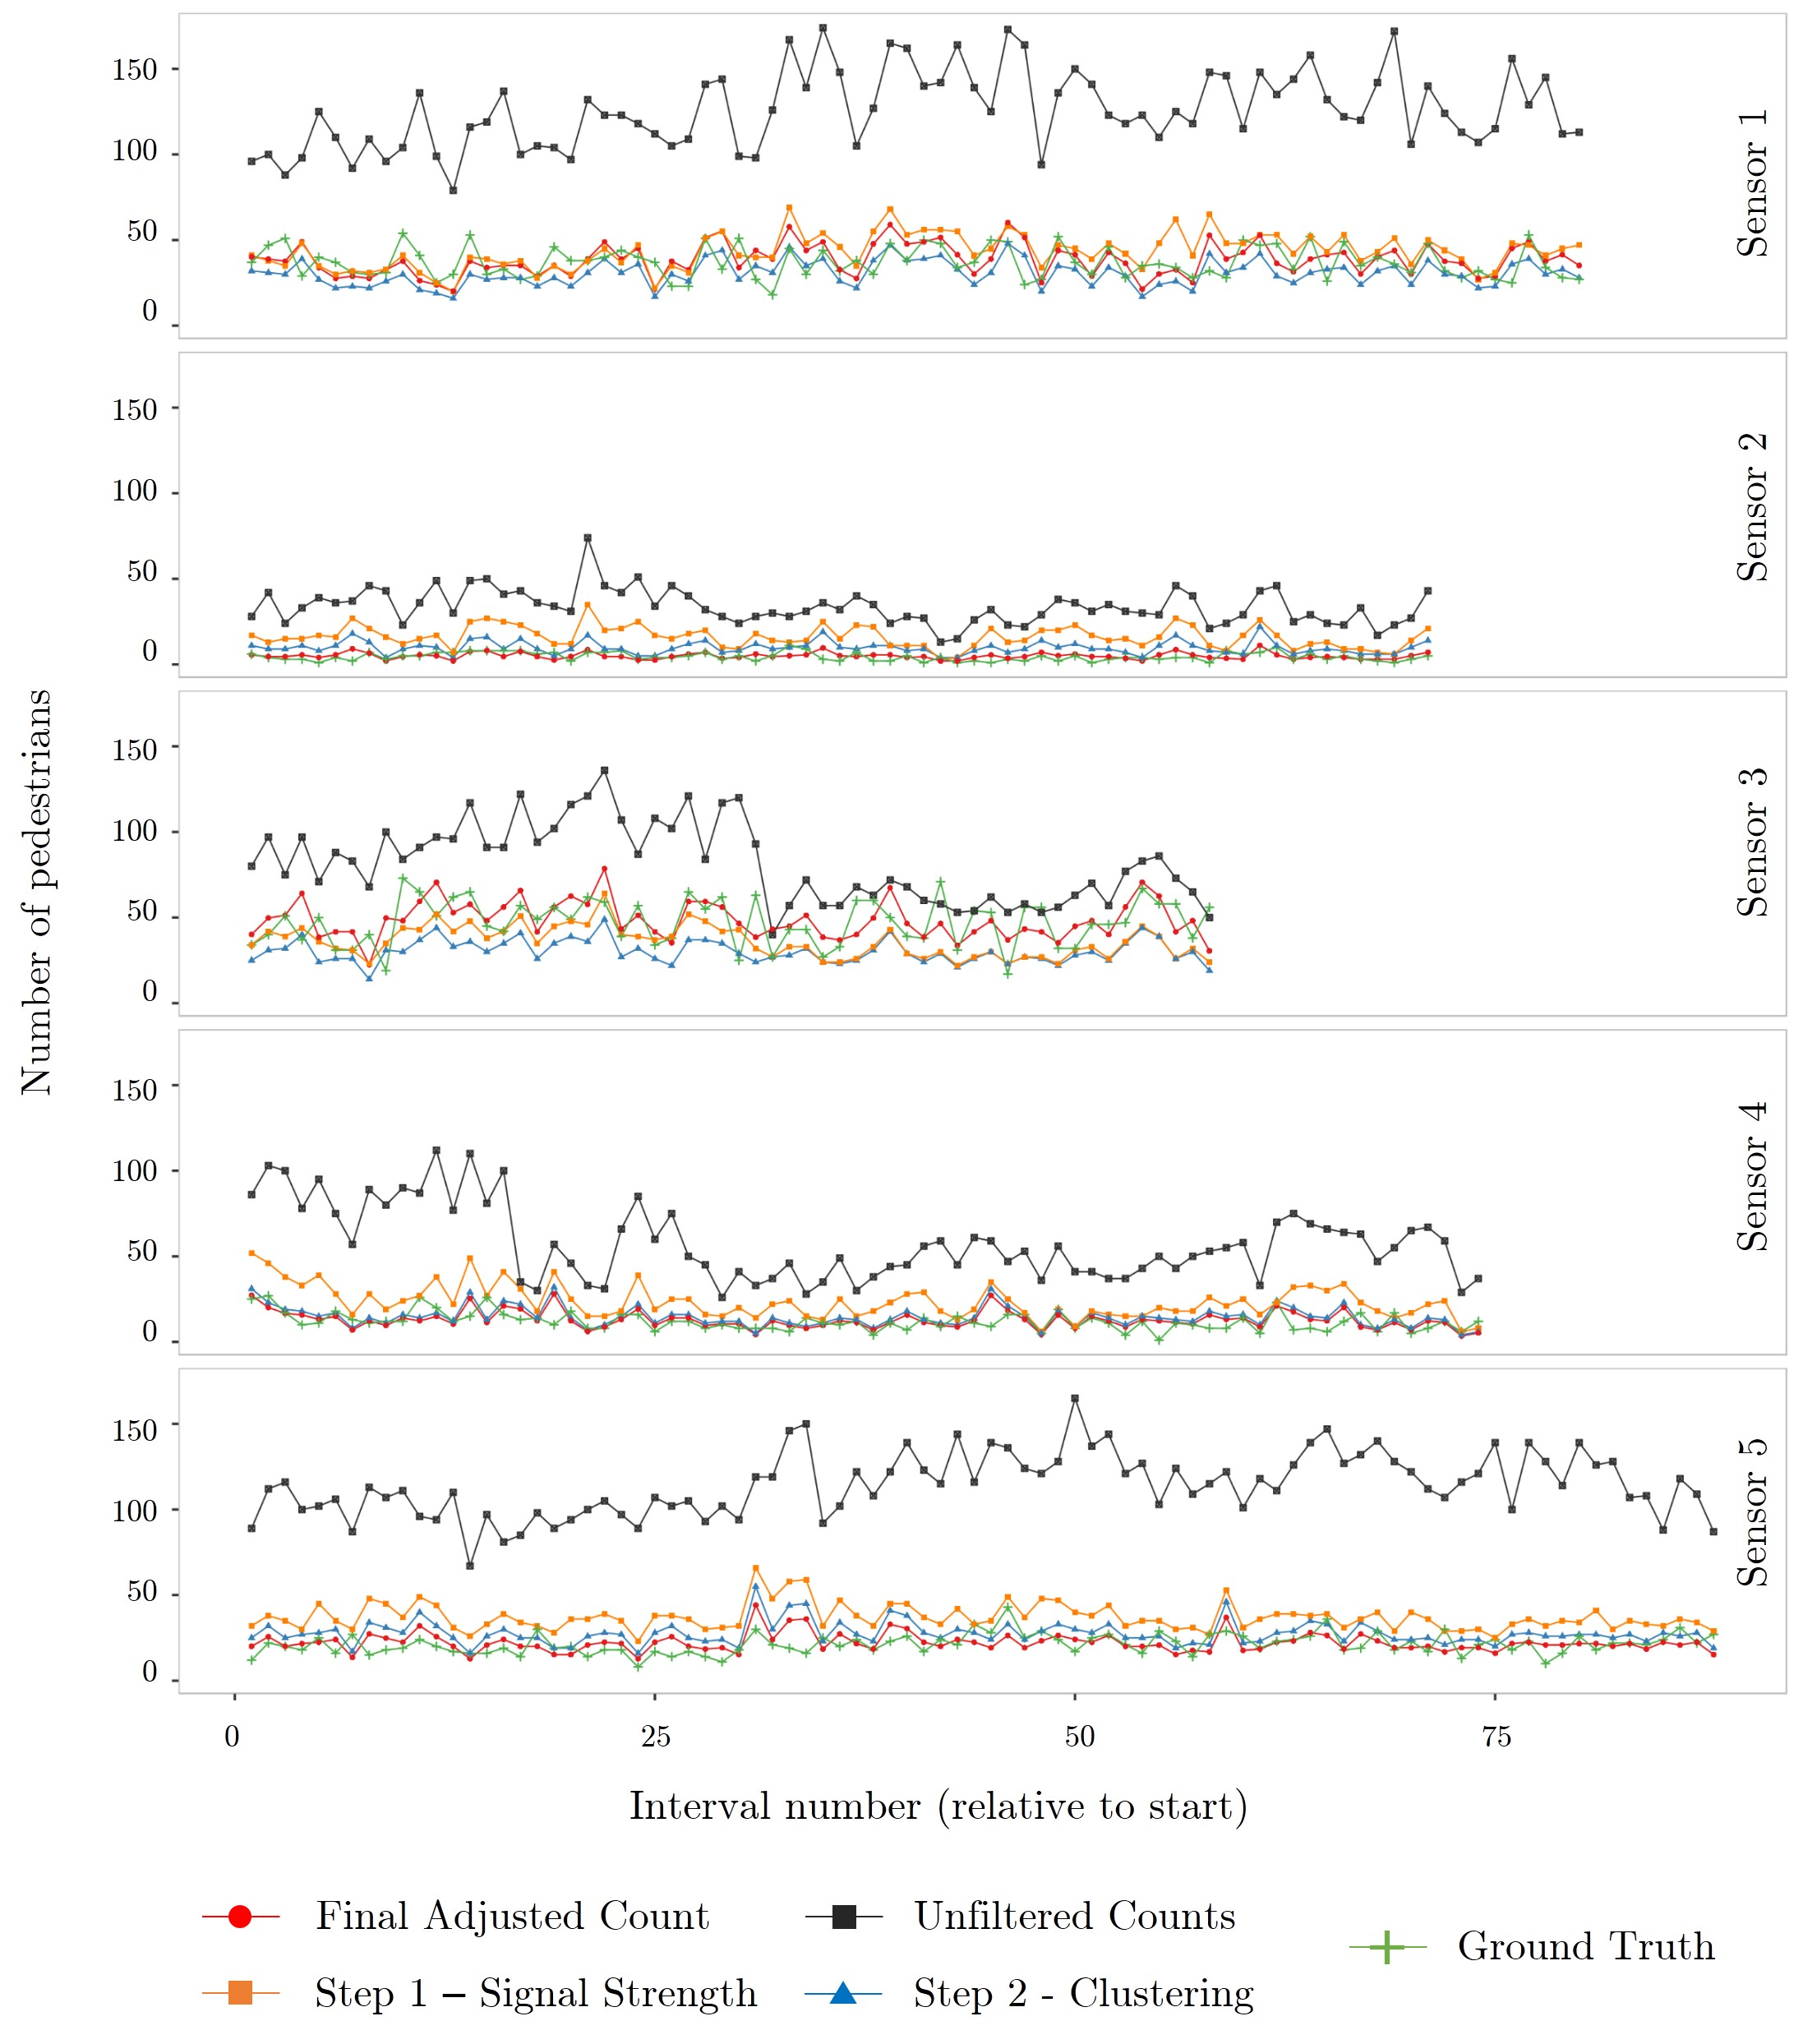
\includegraphics [width=\linewidth,trim=6 6 6 6,clip] {images/main_comparison.jpeg}
		\caption{Comparison of all the counts in teh sensors}
		\label{main_comparison}
	\end{center}
\end{figure}


